\documentclass[aspectratio=169,10pt]{beamer}
\usepackage[T1]{fontenc}
\usepackage{lmodern}
\usepackage{amsmath,amssymb}
\usepackage{booktabs,tabularx}
\usepackage{graphicx}
\usepackage{tikz}
\usepackage{siunitx}
\usepackage{hyperref}
\usetikzlibrary{arrows.meta,decorations.pathmorphing}

\definecolor{ink}{HTML}{17313D}
\definecolor{accent}{HTML}{00677A}
\definecolor{warm}{HTML}{B44A25}
\definecolor{soft}{HTML}{E9F2F3}
\definecolor{muted}{HTML}{52636A}
\setbeamercolor{normal text}{fg=ink,bg=white}
\setbeamercolor{structure}{fg=accent}
\setbeamercolor{frametitle}{fg=ink,bg=white}
\setbeamerfont{frametitle}{series=\bfseries,size=\Large}
\setbeamerfont{title}{series=\bfseries,size=\Huge}
\setbeamerfont{subtitle}{size=\large}
\setbeamertemplate{navigation symbols}{}
\setbeamertemplate{itemize item}{\color{accent}$\bullet$}
\setbeamertemplate{footline}{\hbox{\begin{beamercolorbox}[wd=.86\paperwidth,ht=2.7ex,dp=1ex,leftskip=.45cm]{normal text}\scriptsize Advanced Control Theory \quad | \quad Quarter-car AFC paper analysis\end{beamercolorbox}\begin{beamercolorbox}[wd=.14\paperwidth,ht=2.7ex,dp=1ex,rightskip=.45cm plus1fil]{normal text}\hfill\scriptsize\insertframenumber/\inserttotalframenumber\end{beamercolorbox}}}
\addtobeamertemplate{frametitle}{}{\vspace{-0.6em}\textcolor{accent}{\rule{\linewidth}{0.7pt}}}
\sisetup{detect-all,per-mode=symbol}

\newcommand{\source}[1]{\vfill{\color{muted}\scriptsize #1}}
\newcommand{\takeaway}[1]{\vfill\begin{beamercolorbox}[wd=\linewidth,sep=1ex]{block body}\color{accent}\bfseries #1\end{beamercolorbox}}

\title{Approximation-Free Active Suspension Control}
\subtitle{Na et al. (2022): paper analysis and MATLAB/Simulink reproduction}
\author{Advanced Control Theory course project}
\date{30 September 2026}

\begin{document}

\begin{frame}[plain]
\vspace{0.6cm}
{\color{accent}\rule{2.0cm}{1.2pt}}\par\vspace{0.4cm}
{\usebeamerfont{title}\inserttitle\par}
\vspace{0.4cm}
{\usebeamerfont{subtitle}\insertsubtitle\par}
\vspace{0.45cm}
\textcolor{muted}{\insertauthor}\par
\vspace{0.2cm}
\textcolor{muted}{\insertdate}
\vfill
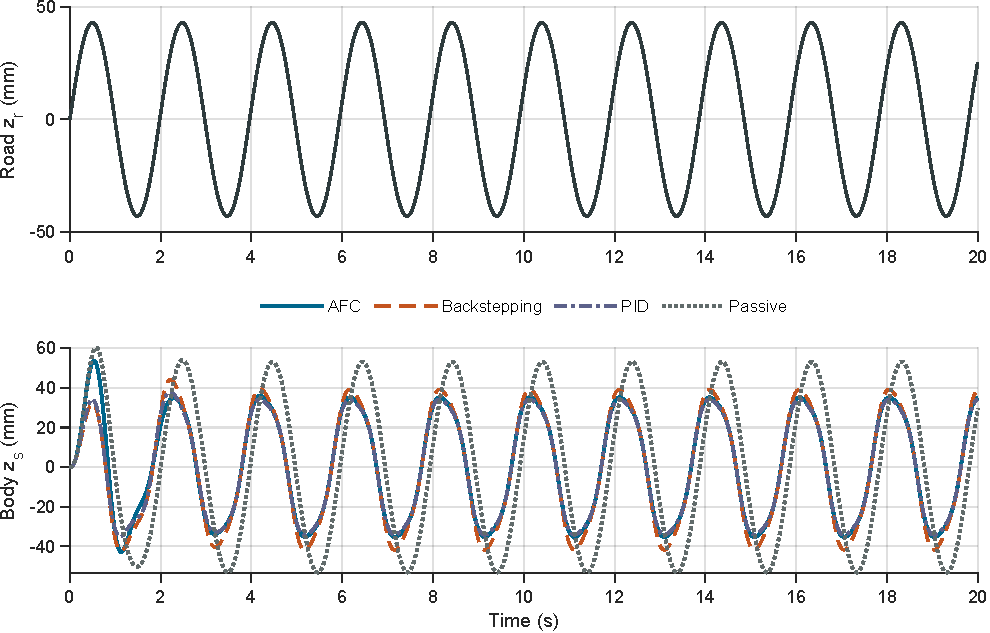
\includegraphics[width=0.80\linewidth,height=1.75cm,keepaspectratio]{paper_assets/response_comparison.pdf}
\end{frame}

\begin{frame}{Research question}
\vspace{0.25cm}
\begin{columns}[T,totalwidth=\linewidth]
\begin{column}{0.50\linewidth}
{\color{accent}\large\bfseries Objective}\par\vspace{0.15cm}
Reduce body vibration under road disturbance while keeping a prescribed transient bound and feasible hydraulic command.
\vspace{0.5cm}

{\color{accent}\large\bfseries Paper method}\par\vspace{0.15cm}
Three-stage approximation-free control (AFC), with a shrinking prescribed-performance function (PPF) and transformed errors.
\end{column}
\begin{column}{0.44\linewidth}
{\color{warm}\large\bfseries Our reproduction question}\par\vspace{0.15cm}
What can we verify from published equations and road cases when the original rig constants and raw signals are unavailable?
\vspace{0.5cm}

{\color{warm}\large\bfseries Evidence boundary}\par\vspace{0.15cm}
The figures here are a representative simulation, not a digitized or reconstructed hardware experiment.
\end{column}
\end{columns}
\source{Source paper: J. Na et al., IEEE TSMC: Systems 52(8), 4714--4726, 2022. DOI: 10.1109/TSMC.2021.3103807.}
\end{frame}

\begin{frame}{Physical system and model}
\begin{columns}[c,totalwidth=\linewidth]
\begin{column}{0.43\linewidth}
\centering
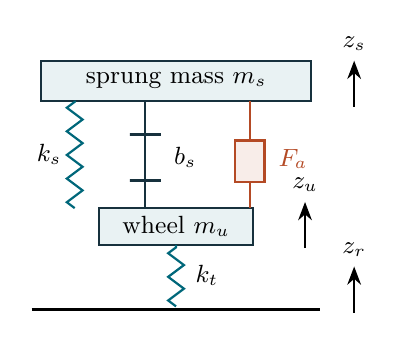
\begin{tikzpicture}[x=0.78cm,y=0.78cm,>=Stealth,thick,every node/.style={font=\small}]
  \draw[fill=soft,draw=ink] (1.4,3.7) rectangle (5.8,4.35);
  \node at (3.6,4.02) {sprung mass $m_s$};
  \draw[fill=soft,draw=ink] (2.35,1.35) rectangle (4.85,1.95);
  \node at (3.6,1.65) {wheel $m_u$};
  \draw[decorate,decoration={zigzag,segment length=3mm,amplitude=1mm},draw=accent] (1.95,1.95)--(1.95,3.7);
  \node[left] at (1.9,2.83) {$k_s$};
  \draw[draw=ink] (3.1,1.95)--(3.1,2.4)--(2.85,2.4)--(3.35,2.4);
  \draw[draw=ink] (3.1,2.4)--(3.1,3.15)--(2.85,3.15)--(3.35,3.15);
  \draw[draw=ink] (3.1,3.15)--(3.1,3.7);
  \node[right] at (3.4,2.78) {$b_s$};
  \draw[draw=warm] (4.8,1.95)--(4.8,2.38);
  \draw[draw=warm,fill=warm!10] (4.56,2.38) rectangle (5.04,3.05);
  \draw[draw=warm] (4.8,3.05)--(4.8,3.7);
  \node[right,text=warm] at (5.1,2.75) {$F_a$};
  \draw[decorate,decoration={zigzag,segment length=3mm,amplitude=1mm},draw=accent] (3.6,0.35)--(3.6,1.35);
  \node[right] at (3.75,0.85) {$k_t$};
  \draw (1.25,0.3)--(5.95,0.3);
  \draw[->] (6.5,3.6)--(6.5,4.35) node[above] {$z_s$};
  \draw[->] (5.7,1.3)--(5.7,2.05) node[above] {$z_u$};
  \draw[->] (6.5,0.25)--(6.5,1.0) node[above] {$z_r$};
\end{tikzpicture}
\end{column}
\begin{column}{0.52\linewidth}
\begin{align*}
F_s&=k_s(z_s-z_u)+k_{sn}(z_s-z_u)^3\\
F_d&=b_s(\dot z_s-\dot z_u)\\[0.3em]
m_s\ddot z_s&=-F_s-F_d+F_a\\
m_u\ddot z_u&=F_s+F_d-F_t-F_b-F_a
\end{align*}
\vspace{0.25cm}
\(F_a=A P_L\), \quad \(x_5=\kappa P_L\)
\end{column}
\end{columns}
\source{Original schematic and model equations; nonlinear spring and tire damping are set to zero in the numerical experiment.}
\end{frame}

\begin{frame}{Prescribed performance transforms a constraint}
\vspace{0.25cm}
\begin{align*}
\mu_i(t)&=(\mu_{i0}-\mu_{i\infty})e^{-\alpha_i t}+\mu_{i\infty}\\[0.35em]
-\delta\mu_i(t)&<e_i(t)<\bar\delta\mu_i(t)\\[0.35em]
\zeta_i&=\frac{e_i}{\mu_i},\qquad
\epsilon_i=\frac12\ln\!\left(\frac{\delta+\zeta_i}{\bar\delta-\zeta_i}\right)
\end{align*}
\vspace{0.35cm}
\begin{tabularx}{\linewidth}{@{}lX@{}}
\toprule
\(\mu_{i0}\) & initial admissible error\\
\(\alpha_i\) & contraction speed\\
\(\mu_{i\infty}\) & long-run error allowance\\
\bottomrule
\end{tabularx}
\takeaway{A bounded transformed error is the route to staying inside the shrinking envelope.}
\end{frame}

\begin{frame}{Approximation-free recursive law}
\vspace{0.2cm}
\begin{align*}
e_1=x_1 &\quad\longrightarrow\quad u_1=-k_1\epsilon_1\\[0.45em]
e_2=x_2-u_1 &\quad\longrightarrow\quad u_2=-k_2\epsilon_2\\[0.45em]
e_3=x_5-u_2 &\quad\longrightarrow\quad u=-k_3\epsilon_3
\end{align*}
\vspace{0.5cm}
\centering
\begin{tabular}{@{}lrrrr@{}}
\toprule
Case A channel & \(\mu_{i0}\) & \(\mu_{i\infty}\) & \(\alpha_i\) & \(k_i\)\\
\midrule
Displacement & 0.2 & 0.018 & 3 & 25.5\\
Virtual velocity & 110 & 90 & 2 & 12\\
Pressure state & 100 & 80 & 2 & 216\\
\bottomrule
\end{tabular}
\source{Case A values: Na et al. Symmetric \(\delta=\bar\delta=1\) is a project inference, not a published numeric setting.}
\end{frame}

\begin{frame}{What the paper actually reports}
\vspace{0.4cm}
\begin{tabularx}{\linewidth}{@{}p{0.34\linewidth}X@{}}
\toprule
Hardware protocol & 50\,Hz real-time control, hydraulic valve limited to \(\pm5\)\,V\\
Fixed-waveform AFC & body acceleration RMS 1.6651\,m/s\(^2\); peak 7.21\,m/s\(^2\)\\
Mean computation & AFC 4.2\,ms; BSC 5.8\,ms; PID 2.6\,ms\\
Other road trials & eight sinusoidal conditions, with case-specific gain adjustments for several slower cases\\
\bottomrule
\end{tabularx}
\vspace{0.65cm}
\textcolor{warm}{\bfseries Important:} the fixed-waveform hardware acceleration statistics cannot be numerically compared with our 10-peak sinusoidal simulation.
\source{All values on this slide are paper-reported, not generated by this project.}
\end{frame}

\begin{frame}{Simulink: sampled AFC and command log}
\centering
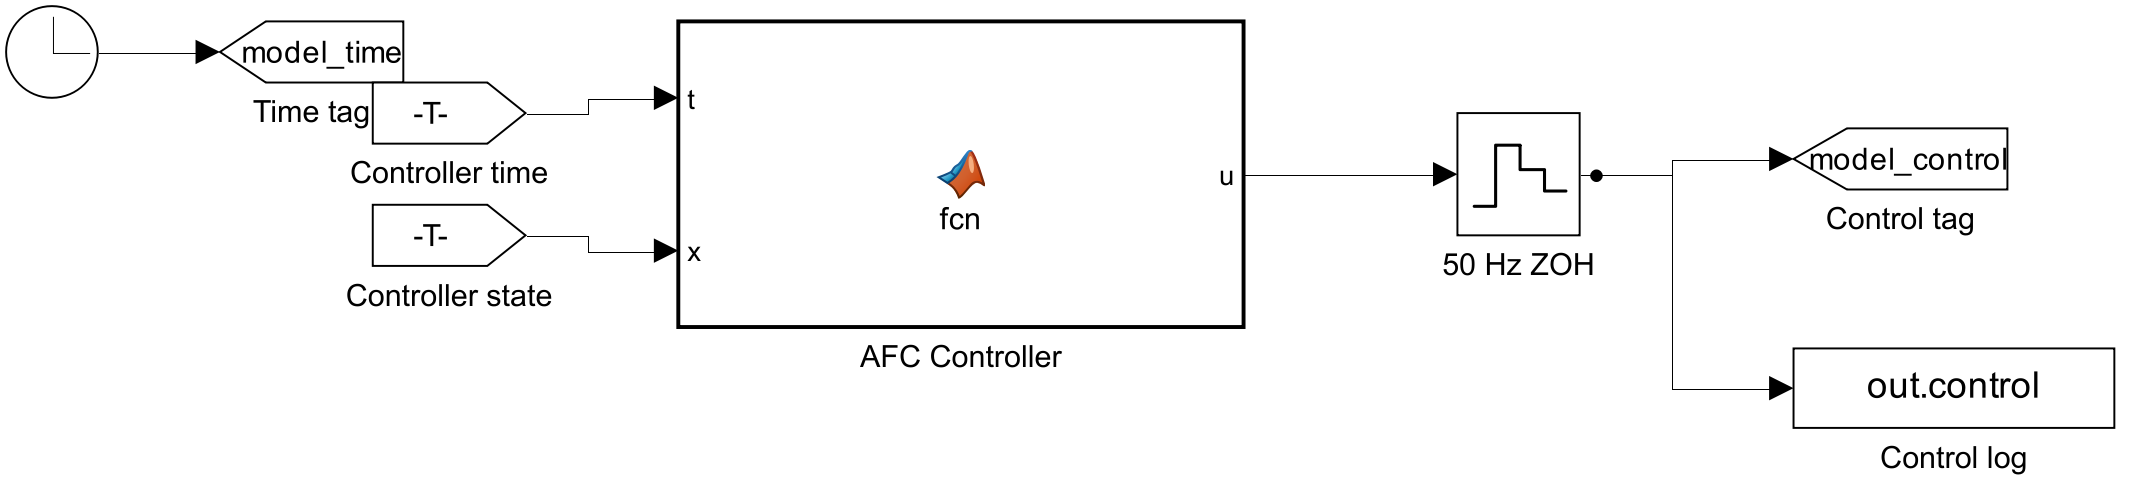
\includegraphics[width=0.94\linewidth,height=0.68\textheight,keepaspectratio]{paper_assets/simulink_control_row.png}\par
\vspace{0.2cm}
\raggedright\small Controller time and state feed the AFC MATLAB Function block; the 50\,Hz zero-order hold applies and logs the valve command.
\source{Top crop of the actual executable \texttt{QuarterCar\_AFC\_Replication.slx} model.}
\end{frame}

\begin{frame}{Simulink: quarter-car plant and feedback}
\centering
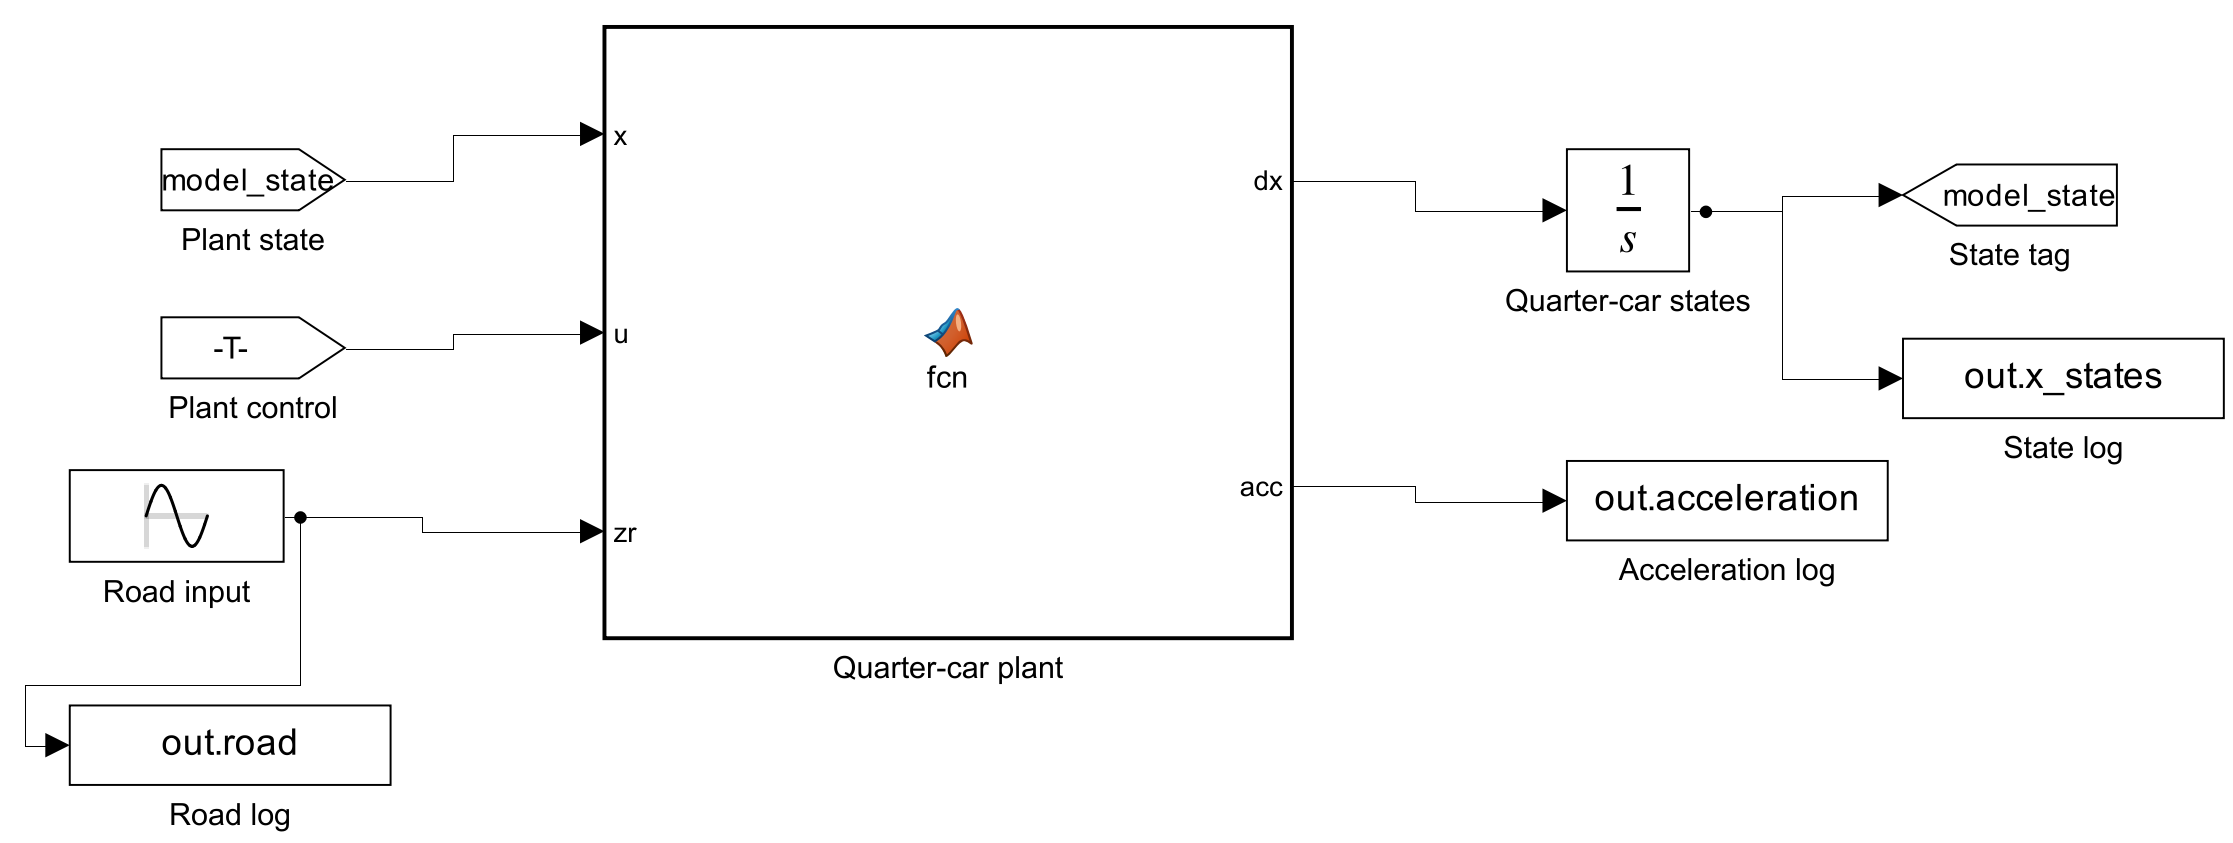
\includegraphics[width=0.94\linewidth,height=0.68\textheight,keepaspectratio]{paper_assets/simulink_plant_row.png}\par
\vspace{0.2cm}
\raggedright\small The plant computes state derivatives and body acceleration; the integrator closes the feedback loop. Road, states, and acceleration are logged.
\source{Bottom crop of the same Simulink model export.}
\end{frame}

\begin{frame}{Parameter ledger: known versus assumed}
\vspace{0.25cm}
\begin{tabularx}{\linewidth}{@{}p{0.28\linewidth}p{0.26\linewidth}X@{}}
\toprule
Quantity & Simulation value & Status\\
\midrule
\(m_s,m_u\) & 320, 40\,kg & representative external quarter-car set\\
\(k_s,k_t,b_s\) & 18, 200\,kN/m; 1\,kN\,s/m & same separate literature set\\
\(A,\beta,P_{\max}\) & \(3.35\times10^{-4}\)\,m\(^2\); 1\,s\(^{-1}\); 10.3425\,MPa & illustrative actuator values\\
\(\kappa,c_{\rm rel},b_u\) & \(10^{-6}\), 0.05, 0.75 & configurable project assumptions\\
50\,Hz; \(\pm5\)\,V & 0.02\,s; \(\pm5\)\,V & retained from source paper\\
\bottomrule
\end{tabularx}
\takeaway{The real rig's valve coefficients and raw signals are the main missing inputs for quantitative replication.}
\end{frame}

\begin{frame}{Experiment reproduced in MATLAB}
\begin{columns}[T,totalwidth=\linewidth]
\begin{column}{0.48\linewidth}
{\color{accent}\large\bfseries Case 10 road}\par
\[z_r(t)=0.043\sin(2\pi\cdot0.505t)\ \mathrm{m}\]
20\,s horizon, 10 peaks; sample time 0.02\,s.
\vspace{0.5cm}

{\color{accent}\large\bfseries Integration}\par
MATLAB: four RK4 substeps per control interval.\par
Simulink: fixed-step \texttt{ode4}, 0.001\,s.
\end{column}
\begin{column}{0.46\linewidth}
{\color{warm}\large\bfseries Comparators}\par
AFC, backstepping, PID, and passive suspension for Case 10.
\vspace{0.5cm}

{\color{warm}\large\bfseries Diagnostics}\par
IAE, ITAE, ITSE, acceleration RMS, voltage clipping, and PPF violation; AFC sweep across all eight published sinusoidal inputs.
\end{column}
\end{columns}
\source{The model uses full simulated state feedback and a surrogate hydraulic pressure-state equation.}
\end{frame}

\begin{frame}{MATLAB figure capture: road and body response}
\centering
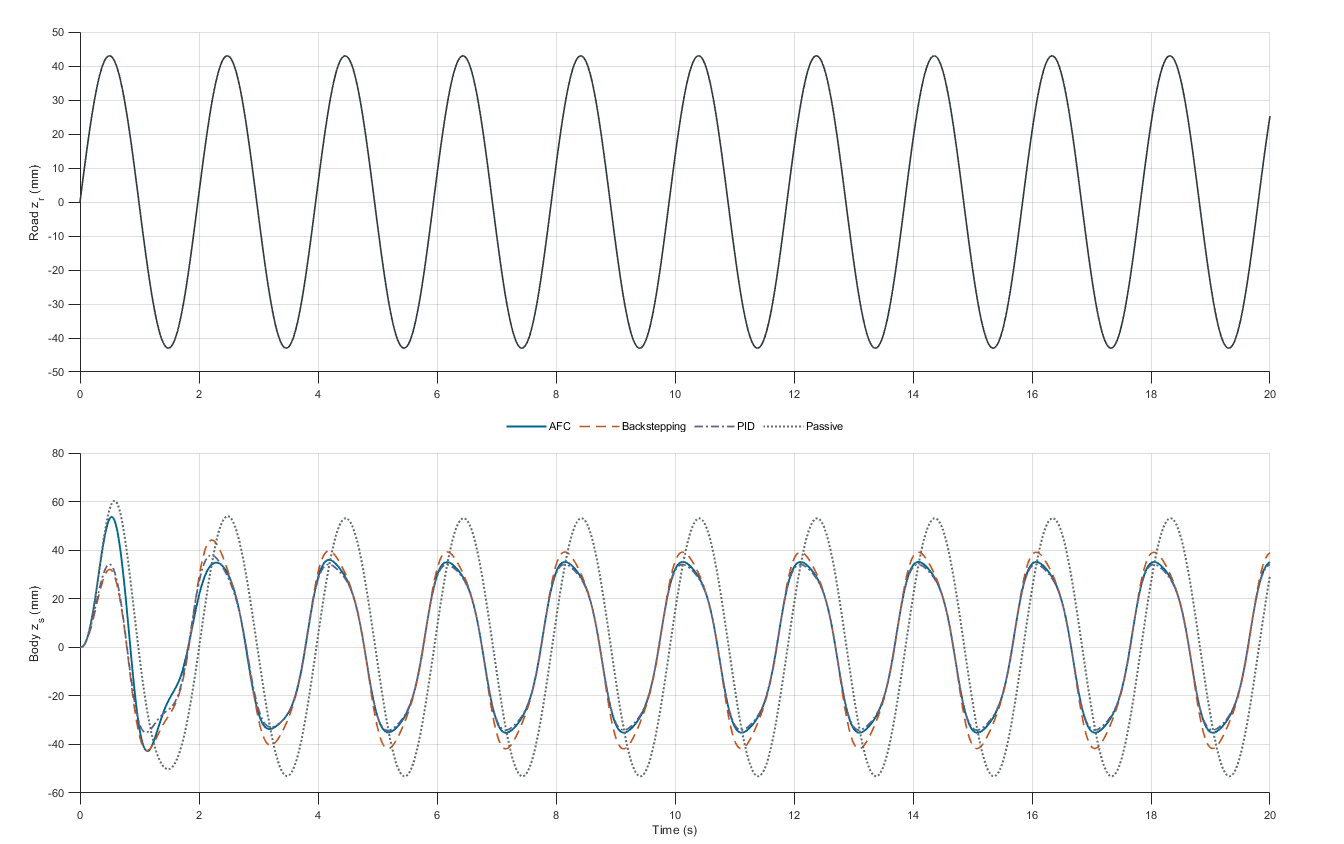
\includegraphics[width=0.92\linewidth,height=0.65\textheight,keepaspectratio]{paper_assets/matlab_figure_capture.png}\par
\vspace{0.2cm}
\raggedright\small Model output: active control improves displacement relative to passive suspension, but PID narrowly leads AFC under these assumptions.
\end{frame}

\begin{frame}{AFC does not retain the assumed PPF}
\centering
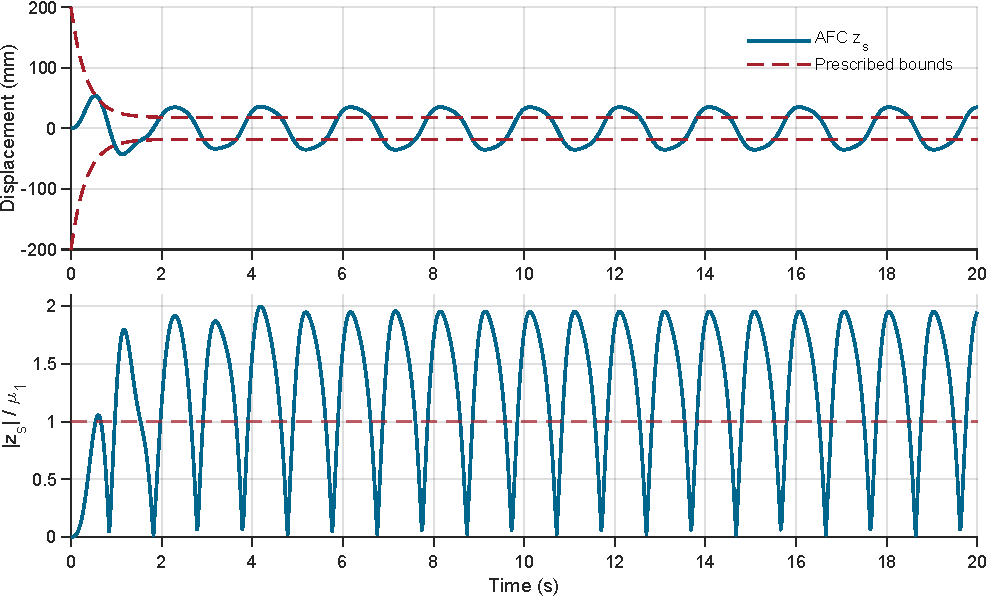
\includegraphics[width=0.92\linewidth,height=0.67\textheight,keepaspectratio]{paper_assets/ppf_audit.pdf}\par
\vspace{0.2cm}
\raggedright\small The normalized ratio \(|z_s|/\mu_1\) exceeds 1; maximum envelope violation is 0.01885\,m.
\end{frame}

\begin{frame}{Actuator authority is the key diagnostic}
\centering
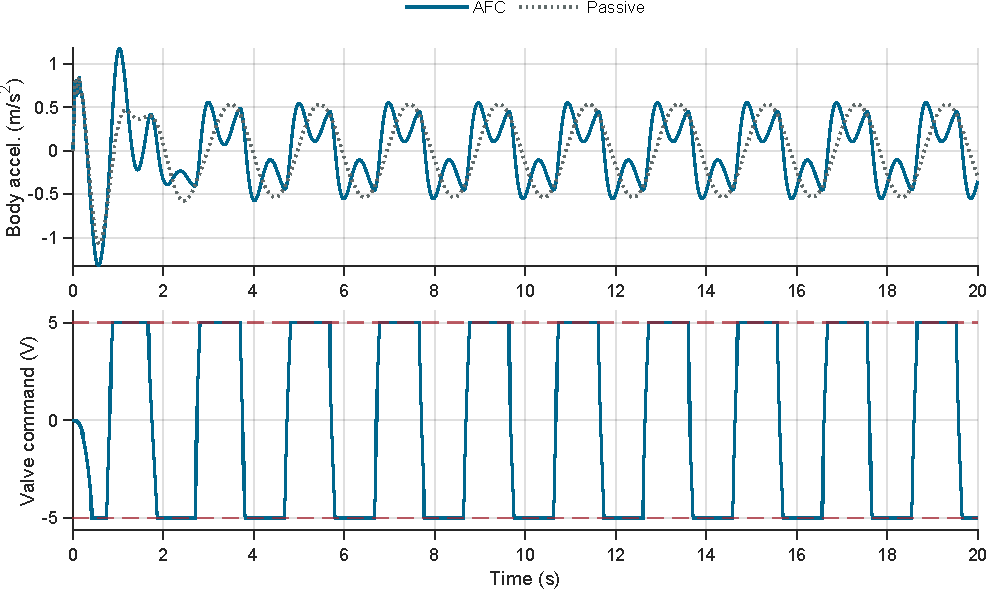
\includegraphics[width=0.92\linewidth,height=0.67\textheight,keepaspectratio]{paper_assets/acceleration_control.pdf}\par
\vspace{0.2cm}
\raggedright\small The raw AFC command exceeds the \(\pm5\)\,V rail in 85.4\% of samples; the plant receives the clipped command.
\end{frame}

\begin{frame}{Controller ranking in the assumed model}
\centering
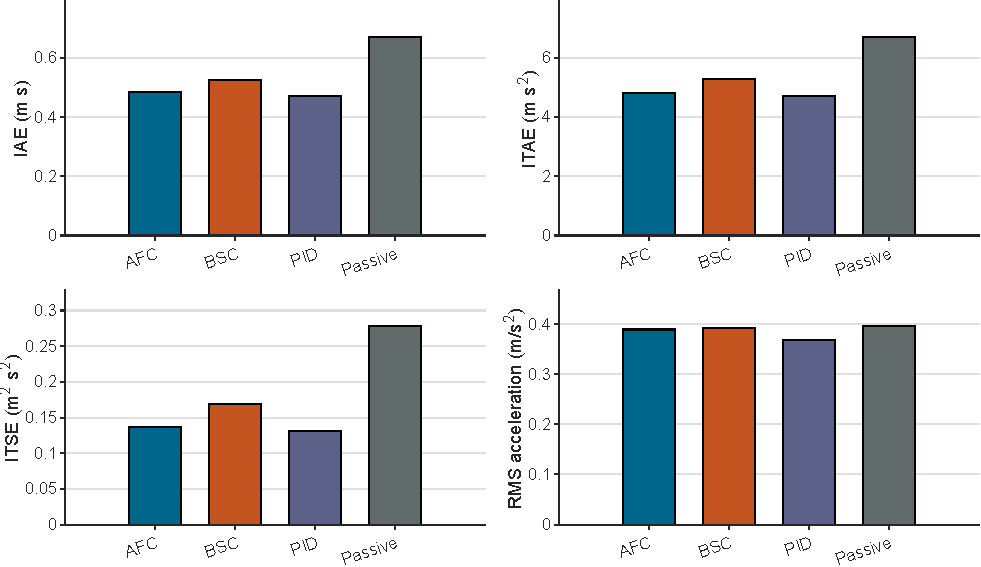
\includegraphics[width=0.92\linewidth,height=0.67\textheight,keepaspectratio]{paper_assets/metric_comparison.pdf}\par
\vspace{0.2cm}
\raggedright\small AFC IAE = 0.4849\,m\,s; passive IAE = 0.6709\,m\,s. PID is lower at 0.4698\,m\,s.
\end{frame}

\begin{frame}{Eight published road inputs, fixed AFC tuning}
\centering
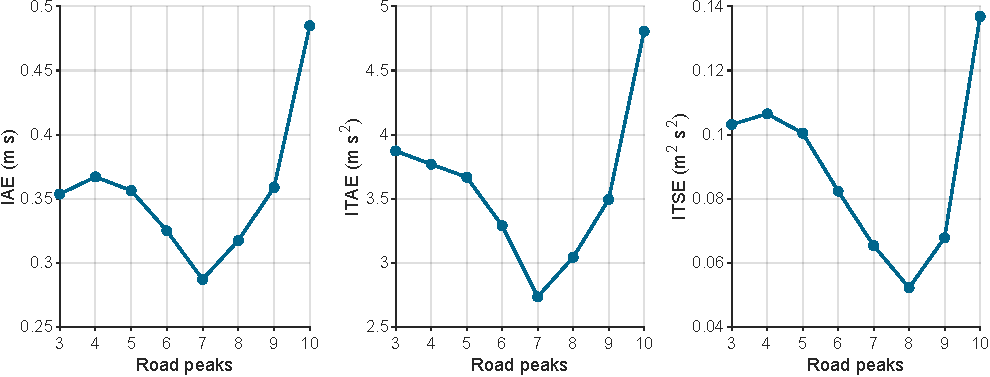
\includegraphics[width=0.94\linewidth,height=0.65\textheight,keepaspectratio]{paper_assets/road_sweep.pdf}\par
\vspace{0.2cm}
\raggedright\small The simulated indices are non-monotonic. The paper retunes several slower cases; this project deliberately holds Case A gains fixed to expose road sensitivity.
\end{frame}

\begin{frame}{Independent numerical implementation check}
\centering
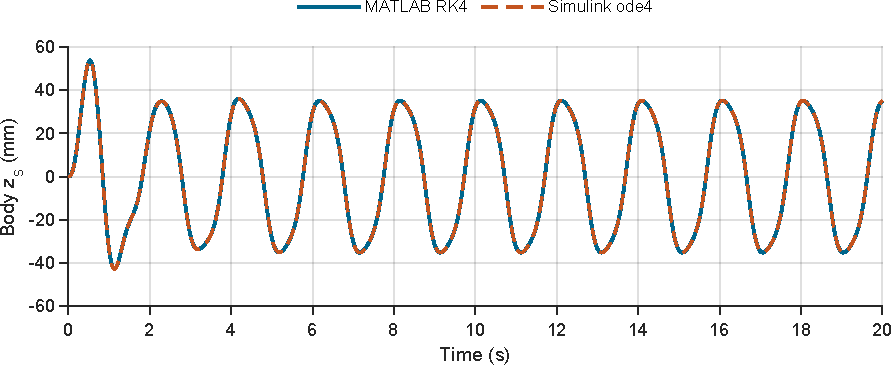
\includegraphics[width=0.93\linewidth,height=0.65\textheight,keepaspectratio]{paper_assets/implementation_crosscheck.pdf}\par
\vspace{0.2cm}
\raggedright\small MATLAB and Simulink agree to a maximum body-displacement difference of \(2.10\times10^{-8}\)\,m for the 10-peak run. This validates code consistency, not physical parameter identification.
\end{frame}

\begin{frame}{Conclusion and next validation step}
\vspace{0.2cm}
\begin{tabularx}{\linewidth}{@{}p{0.30\linewidth}X@{}}
\toprule
What is reproduced & AFC recursion, PPF settings, 50\,Hz sampled control, sinusoidal road cases, and independent MATLAB/Simulink traces.\\
What is not reproduced & Original rig/valve identification, fixed-waveform samples, sensor/observer path, and hardware measurements.\\
What the model reveals & Reduced error versus passive, but severe voltage saturation and PPF violation for Case 10.\\
\bottomrule
\end{tabularx}
\vspace{0.45cm}
\textcolor{accent}{\bfseries Next:} identify the hydraulic actuator and obtain the source waveform/time series before claiming quantitative experimental agreement.
\source{Code, model, plots, report, and slides: \url{https://github.com/Galabavamsi/quarter-car-afc-replication}.}
\end{frame}

\begin{frame}{References}
\small
\begin{thebibliography}{9}
\bibitem{na} J. Na et al., ``Active Suspension Control of Quarter-Car System With Experimental Validation,'' \emph{IEEE TSMC: Systems}, 52(8), 4714--4726, 2022. \href{https://doi.org/10.1109/TSMC.2021.3103807}{doi:10.1109/TSMC.2021.3103807}.
\bibitem{jin} P. Jin, W. Xue, and K. Li, ``Actuator Fault Estimation for Vehicle Active Suspensions Based on Adaptive Observer and Genetic Algorithm,'' \emph{Shock and Vibration}, 2019. \href{https://doi.org/10.1155/2019/1783850}{doi:10.1155/2019/1783850}.
\bibitem{abdulzahra} A. K. Abdulzahra and T. Y. Abdalla, ``Fuzzy Sliding Mode Control Scheme for Vehicle Active Suspension System Optimized by ABC Algorithm,'' \emph{IJISA}, 11(12), 1--10, 2019. \href{https://doi.org/10.5815/ijisa.2019.12.01}{doi:10.5815/ijisa.2019.12.01}.
\end{thebibliography}
\end{frame}

\end{document}
